%% BioMed_Central_Tex_Template_v1.06
%%                                      %
%  bmc_article.tex            ver: 1.06 %
%                                       %

%%IMPORTANT: do not delete the first line of this template
%%It must be present to enable the BMC Submission system to
%%recognise this template!!

%%%%%%%%%%%%%%%%%%%%%%%%%%%%%%%%%%%%%%%%%
%%                                     %%
%%  LaTeX template for BioMed Central  %%
%%     journal article submissions     %%
%%                                     %%
%%          <8 June 2012>              %%
%%                                     %%
%%                                     %%
%%%%%%%%%%%%%%%%%%%%%%%%%%%%%%%%%%%%%%%%%


%%%%%%%%%%%%%%%%%%%%%%%%%%%%%%%%%%%%%%%%%%%%%%%%%%%%%%%%%%%%%%%%%%%%%
%%                                                                 %%
%% For instructions on how to fill out this Tex template           %%
%% document please refer to Readme.html and the instructions for   %%
%% authors page on the biomed central website                      %%
%% http://www.biomedcentral.com/info/authors/                      %%
%%                                                                 %%
%% Please do not use \input{...} to include other tex files.       %%
%% Submit your LaTeX manuscript as one .tex document.              %%
%%                                                                 %%
%% All additional figures and files should be attached             %%
%% separately and not embedded in the \TeX\ document itself.       %%
%%                                                                 %%
%% BioMed Central currently use the MikTex distribution of         %%
%% TeX for Windows) of TeX and LaTeX.  This is available from      %%
%% http://www.miktex.org                                           %%
%%                                                                 %%
%%%%%%%%%%%%%%%%%%%%%%%%%%%%%%%%%%%%%%%%%%%%%%%%%%%%%%%%%%%%%%%%%%%%%

%%% additional documentclass options:
%  [doublespacing]
%  [linenumbers]   - put the line numbers on margins

%%% loading packages, author definitions

\documentclass[twocolumn]{bmcart}% uncomment this for twocolumn layout and comment line below
%\documentclass{bmcart}

%%% Load packages
%\usepackage{amsthm,amsmath}
%\RequirePackage{natbib}
\RequirePackage{hyperref}
\usepackage[utf8]{inputenc} %unicode support
%\usepackage[applemac]{inputenc} %applemac support if unicode package fails
%\usepackage[latin1]{inputenc} %UNIX support if unicode package fails


%%%%%%%%%%%%%%%%%%%%%%%%%%%%%%%%%%%%%%%%%%%%%%%%%
%%                                             %%
%%  If you wish to display your graphics for   %%
%%  your own use using includegraphic or       %%
%%  includegraphics, then comment out the      %%
%%  following two lines of code.               %%
%%  NB: These line *must* be included when     %%
%%  submitting to BMC.                         %%
%%  All figure files must be submitted as      %%
%%  separate graphics through the BMC          %%
%%  submission process, not included in the    %%
%%  submitted article.                         %%
%%                                             %%
%%%%%%%%%%%%%%%%%%%%%%%%%%%%%%%%%%%%%%%%%%%%%%%%%


%\def\includegraphic{}
%\def\includegraphics{}
\usepackage{graphicx}


%%% Put your definitions there:
\startlocaldefs
\endlocaldefs

% Our variable names
\newcommand{\chrOnePop}{Chr19\_Population}
\newcommand{\FullPop}{Full\_Population}
\newcommand{\FullFam}{Chr1\_Family}


%%% Begin ...
\begin{document}

%%% Start of article front matter
\begin{frontmatter}

\begin{fmbox}
\dochead{Methodology}

%%%%%%%%%%%%%%%%%%%%%%%%%%%%%%%%%%%%%%%%%%%%%%
%%                                          %%
%% Enter the title of your article here     %%
%%                                          %%
%%%%%%%%%%%%%%%%%%%%%%%%%%%%%%%%%%%%%%%%%%%%%%

\title{Scalable Clustering of Genotype Information using MapReduce}

%%%%%%%%%%%%%%%%%%%%%%%%%%%%%%%%%%%%%%%%%%%%%%
%%                                          %%
%% Enter the authors here                   %%
%%                                          %%
%% Specify information, if available,       %%
%% in the form:                             %%
%%   <key>={<id1>,<id2>}                    %%
%%   <key>=                                 %%
%% Comment or delete the keys which are     %%
%% not used. Repeat \author command as much %%
%% as required.                             %%
%%                                          %%
%%%%%%%%%%%%%%%%%%%%%%%%%%%%%%%%%%%%%%%%%%%%%%

\author[
   addressref={aff1,aff2},                   % id's of addresses, e.g. {aff1,aff2}
%   noteref={n1},                        % id's of article notes, if any
   email={Aidan.O'Brien@csiro.au}   % email address
]{\inits{AR}\fnm{Aidan R} \snm{O'Brien}}
\author[
   addressref={aff3, aff4},
   email={f.buske@garvan.org.au}
]{\inits{FA}\fnm{Fabian A} \snm{Buske}}
\author[
   addressref={aff1},
   corref={aff1},                       % id of corresponding address, if any
   email={Denis.Bauer@CSIRO.au}
]{\inits{DC}\fnm{Denis C} \snm{Bauer}}

%%%%%%%%%%%%%%%%%%%%%%%%%%%%%%%%%%%%%%%%%%%%%%
%%                                          %%
%% Enter the authors' addresses here        %%
%%                                          %%
%% Repeat \address commands as much as      %%
%% required.                                %%
%%                                          %%
%%%%%%%%%%%%%%%%%%%%%%%%%%%%%%%%%%%%%%%%%%%%%%

\address[id=aff1]{%                           % unique id
  \orgname{Division of Computational Informatics, CSIRO}, % university, etc
  \street{11 Julius Av},                     %
  \postcode{2113}                                % post or zip code
  \city{Sydney},                              % city
  \cny{Australia}                                    % country
}
\address[id=aff2]{%
  \orgname{School of Biomedical Sciences and Pharmacy, Faculty of Health},
%  \street{},
  \postcode{2308}
  \city{Newcastle},
  \cny{Australia}
}
\address[id=aff3]{%
  \orgname{Cancer Epigenetics Program, Cancer Research Division, Kinghorn Cancer Centre, Garvan Institute of Medical Research},
  \street{384 Victoria St},
  \postcode{2010}
  \city{Sydney},
  \cny{Australia}
}
\address[id=aff4]{%
  \orgname{UNSW Medicine, University of New South Wales},
%  \street{},
  \postcode{2052}
  \city{Sydney},
  \cny{Australia}
}


%%%%%%%%%%%%%%%%%%%%%%%%%%%%%%%%%%%%%%%%%%%%%%
%%                                          %%
%% Enter short notes here                   %%
%%                                          %%
%% Short notes will be after addresses      %%
%% on first page.                           %%
%%                                          %%
%%%%%%%%%%%%%%%%%%%%%%%%%%%%%%%%%%%%%%%%%%%%%%

%\begin{artnotes}
%\note{Sample of title note}     % note to the article
%\note[id=n1]{Equal contributor} % note, connected to author
%\end{artnotes}

%\end{fmbox}% comment this for two column layout

%%%%%%%%%%%%%%%%%%%%%%%%%%%%%%%%%%%%%%%%%%%%%%
%%                                          %%
%% The Abstract begins here                 %%
%%                                          %%
%% Please refer to the Instructions for     %%
%% authors on http://www.biomedcentral.com  %%
%% and include the section headings         %%
%% accordingly for your article type.       %%
%%                                          %%
%%%%%%%%%%%%%%%%%%%%%%%%%%%%%%%%%%%%%%%%%%%%%%

\begin{abstractbox}

\begin{abstract} % abstract
\parttitle{Background} Processing genomic information from whole genome sequence studies pose computational challenges due to the unprecedented data volume generated, which render transitional approaches insufficient. However, by utilising advancements in modern hardware accelerators and data processing we can provide the means for scalable solutions. We therefore aim to provide the interface between standard genomic data formats and advanced and scalable analysis libraries like Mahout. 
\parttitle{Results} We achieve an XX-fold speedup by using the scalable k-means MapReduce implementation over the equivalent analysis performed in R and YY-fold speedup for PCA, respectively, by comparable accuracy. Due to memory in the R-Implementation the comparison had to be limited to variant data from chromosome 1 only, however we ran the full dataset (aa GB, bb individuals {\`a} cc variants ) through Mahout demonstrating the scalability. 
\parttitle{Conclusions} Using modern compute paradigms is essential to scale to modern genomic research in an efficient sustainable way. 
\end{abstract}

%%%%%%%%%%%%%%%%%%%%%%%%%%%%%%%%%%%%%%%%%%%%%%
%%                                          %%
%% The keywords begin here                  %%
%%                                          %%
%% Put each keyword in separate \kwd{}.     %%
%%                                          %%
%%%%%%%%%%%%%%%%%%%%%%%%%%%%%%%%%%%%%%%%%%%%%%

\begin{keyword}
\kwd{Hadoop}
\kwd{Mahout}
\kwd{Genotype}
\kwd{Clustering}
\kwd{MapReduce}
\end{keyword}

% MSC classifications codes, if any
%\begin{keyword}[class=AMS]
%\kwd[Primary ]{}
%\kwd{}
%\kwd[; secondary ]{}
%\end{keyword}

\end{abstractbox}
%
\end{fmbox}% uncomment this for twcolumn layout

\end{frontmatter}

%%%%%%%%%%%%%%%%%%%%%%%%%%%%%%%%%%%%%%%%%%%%%%
%%                                          %%
%% The Main Body begins here                %%
%%                                          %%
%% Please refer to the instructions for     %%
%% authors on:                              %%
%% http://www.biomedcentral.com/info/authors%%
%% and include the section headings         %%
%% accordingly for your article type.       %%
%%                                          %%
%% See the Results and Discussion section   %%
%% for details on how to create sub-sections%%
%%                                          %%
%% use \cite{...} to cite references        %%
%%  \cite{koon} and                         %%
%%  \cite{oreg,khar,zvai,xjon,schn,pond}    %%
%%  \nocite{smith,marg,hunn,advi,koha,mouse}%%
%%                                          %%
%%%%%%%%%%%%%%%%%%%%%%%%%%%%%%%%%%%%%%%%%%%%%%

%%%%%%%%%%%%%%%%%%%%%%%%% start of article main body
% <put your article body there>

%%%%%%%%%%%%%%%%
%% Background %%
%%
\section*{Background}
Grouping individuals based on the genomic profile is a commonly performed tasks to identify population structure~\cite{Gao2007} or elucidate different haplotype involvement in diseases susceptibility~\cite{Laitman2013}.  Traditionally both the number of individuals and included genotypes, typically from SNP arrays, were relatively small and libraries in Bioconductor sufficient. However, recent technological advances in whole genome sequencing have made population-scale sequencing feasible. It is hence economical to generate studies with sample sizes currently reserved for larger consortia such as the 1000 genomes project~\cite{1KG2012} or TCGA~\cite{TCGA2013}. At the same time, whole genome sequencing enables the inclusion of rare or even somatic mutations in the analysis, increasing the feature space by orders of magnitude. This drastic increase in both sample numbers and features per sample requires a massively parallele approach to data processing. 

As a result of these big data challenges, MapReduce approaches are increasingly being used in bioinformatics (for reviews see~cite{Zou2013, Qiu2010,Taylor2010}). This is especially the case for sequence analysis tasks, such as read mapping~\cite{Schatz2009}, duplicate removal~\cite{Jourdren2012}, and variant calling~\cite{Langmead2009, McKenna2010} or Genome Wide Analysis Study based tasks~\cite{Huang2013, Guo2014}.

At the same time, sophisticated machine learning methodologies are increasingly adapted to utilise MapReduce paradigms overcoming callings that arise due to their iterative nature~\cite{Chu2009}. Specifically, the Mahout project\url{https://mahout.apache.org/} has been developed extensively~\cite{Ranger2007, Owen2011} and was successfully applied in the clinical informatics space~\cite{Dong2013}.

We therefore link the two areas by providing an interface between Mahout and the standard variant data format, VCF~\cite{1KG2012}, which opens up the application of Mahout's different machine learning algorithms to be applied to genotype-based tasks.   
To demonstrate the capability we cluster variant datasets from the 1000 genomes project to determine population structure as well as ancestry using different algorithms available in Mahout. In the first two sections we benchmark the performance and accuracy of Mahout's implementations against standard R based implementations on a reduced version of the data and in the last section we investigate the performance on the full dataset, demonstrating how seamless Mahout can transit to population-scale tasks.   

%SeqWare~{OConnor2010} Libraries \cite{Doering2008,Schumacher2014,Nordberg2013}







\section*{Results and discussion}
\subsection*{Runtime}
We measured the runtime seperately for pre-processing stage as well as the k-means clustering stage. 
Following are the results from the (\chrOnePop) dataset. Pre-processing the data to Mahout's sequence files took approximately 21 minutes (1255s) and used
approximately 1.8GB (1831160kb) physical memory (pmem) and 7.6GB (7646232kb) virtual memory (vmem).
Conversly,  pre-processing the data to R's in memory matrix took approximately 56 minutes (3341s) and used
approximately 17.7GB (17696940kb) pmem and 18GB (18000196kb) vmem. The size of the Mahout sequence file,
which is saved to disk, is 835MB. K-means clustering the data, however, was faster with R, possibly due to the data already being present in memory.
R took 7s, whereas Mahout took 10 minutes.\\
Although the Mahout pipeline was about 25 minutes faster than R's. the clustering step with R was much faster than with Mahout. This is likely due to the additional overhead involved in setting up the Hadoop nodes, spawning the map and reduce instances, and distributing the data between the instances. R on the other hand, already had the data in memory, and only had to process that data. In the case of this comparison, the data set is likely too small to truly reap the benefit of Hadoop's
MapReduce algorithm. The main benefit of mahout in this scenario is the memory consumption. There is nearly a 10-fold increase for Mahout
compared to R. 



\subsection*{Accuracy}
For this example, we knew the correct clusters from 1000 Genomes metadata. This metadata assigns a population and family value to each of the 1092 individuals.
With the foreknowledge of the correct clusters, the Adjusted Rand Index enables us to assign a score to cluster accuracy~\cite{Hubert1985}. 



\subsection*{Real World Example}
Text for this section.



\section*{Conclusion}
Note,  Domain-specific language for linear algebraic operations on top of Apache Spark \url{http://spark.apache.org/}
ADAM~\cite{Massie2013}


\section*{Methods}
\subsection*{Datasets}
We used variant call format (VCF) files from the 1000 Genomes Project.
These VCF files contain information about the genetic variants between each of the 1092 individuals and a reference genome derived from GRCh37. 
Each of the VCF files are partitioned by chromosome.\\
Metadata available from the 1000 Genomes Consortium specifies additional attributes for each individual, including population and familial data.\\
To be able to compare with R, we created a subset of the entire human variant dataset by using only variants from chromosome 1 (\chrOnePop) where we investigate the correct grouping of the population structure. 
The population structure is also investigated using the full dataset, i.e. all chromosomes, using Mahout libraries (\FullPop). 
In addition, we also investigate whether the full dataset allows the accurate prediction of the more detailed family association (\FullFam).
Table~\ref{datasets} contains an overview of the datasets.

\subsection*{Hardware}
We processed the data using a Portable Batch System (PBS) cluster. We allocated one node and 64GB memory for the comparison between Mahout and R.
Each node has eight CPU cores, however both applications run a single thread for pre-processing the data.
For the (\FullPop) dataset, we ran the job on a PBS cluster of x nodes, with twelve CPU cores and 48GB of memory per node.

\subsection*{Pre-processing}
Mahout requires sequence files as input to its clustering algorithms, and it provides libraries for writing vectors to this file format.
Separate vectors for each sample, in this case, an individual, contain entries for each of the sample's features, where each entry is
a \texttt{double}. Although additional samples can subsequently be appended to sequence files, the entire feature-set for each sample must be
appended in a single write operation. Because the features for each sample are present in columns, as tab-separated elements in VCF
files, we recursively transpose the data into CSV files. Each comma-separated row contains the feature-set for a sample,
as well as the sample identity. Concurrently, we convert the values from the VCF file to doubles, as required for Mahout's sequence
file format and the many algorithms this format can serve as input for. We set the value of the double to the Hamming distance between
each variant and the reference genome. Therefore, a value identical to the reference will be 0, a heterozygous variant on either strand
will be 1 and a homozygous variant will be 2.
At this stage, the CSV files from more than one VCF file are concatenated into the one file. This resulting CSV file serves as the input for
a custom Java function. This iterates over the CSV file, extracting the sample name and feature-set from each line, and calls a Mahout
function to store this data as a named \texttt{DenseVector} object. The vectors are populated primarily by zeroes, so we convert this object to 
the more efficient \texttt{SequentialAccessSparseVector} object, which stores only non-zero doubles in an array, and maps their position in a second array.

This object is serialized, and the resulting file can serve as input to the majority of Mahout's algorithms. 



\subsection*{Mahout K-means clustering}
To cluster the samples from the sequence files, we use Mahout 0.9 in conjunction with Hadoop 2.2.0. 
The clustering steps are the same for each dataset, however, due to the increased feature size we designate more memory to the
YARN containers (a container being the resources allocated to each map or reduce iteration). For the first step, we specify \texttt{k},
the number of clusters. The function \texttt{RandomSeedGenerator.buildRandom} creates a new sequence file containing \texttt{k}
random centroids from the samples sequence file. The sequence file
of samples and the sequence file of centroids serve as the input to \texttt{KMeansDriver.run}, a static Mahout API function that launches
a k-means clustering job on the Hadoop service. 


\subsection*{R K-means clustering}
We use `readVcf' from the R library, `VariantAnnotation', to iteratively read in the VCF file. For each iteration, we convert the data to a matrix and
change the values for each variant to the Hamming distance, as mentioned previously. We then transpose the matrix, so individuals are represented
by rows, and append the matrix to that from the previous iteration. Once the matrix contains all of the variants from the VCF file, we cluster the data
using the `kmeans' algorithm from the `stats' library.



\subsection*{Clustering quality}
We scored the clusters with the Adjusted Rand index. 
%TODO: can you provide the formular
This index compares two different cluster sets and assigns a value based on their similarity. The value is zero for independent clusterings and one for identical clusterings. We compared the Mahout k-means
clusters and the R k-means clusters to the known clusters based on meta data from the 1000 genome project. For the known clusters,
individuals were partitioned by their super population code (ASN, EUR, AFR, AMR). 
%TODO: "also on \chrOnePop" on what dataset did you compare the R performance otherwise ?
We also compared the Mahout clusters to the
R clusters for the Chr1 subset data.



\subsection*{Performance}
We recorded the memory usage and run-time from the PBS logs. For the Mahout jobs, we queued separate jobs
for pre-processing and k-means clustering to get an accurate representation of the time and memory requirements for each stage.
For the R job, where we could not easily separate the pre-processing and clustering components, we printed the time between
stages using the function, \texttt{proc.time()}.


%%%%%%%%%%%%%%%%%%%%%%%%%%%%%%%%%%%%%%%%%%%%%%
%%                                          %%
%% Backmatter begins here                   %%
%%                                          %%
%%%%%%%%%%%%%%%%%%%%%%%%%%%%%%%%%%%%%%%%%%%%%%

\begin{backmatter}

\section*{Availability of supporting data}
\section*{List of abbreviations}


\section*{Competing interests}
  The authors declare that they have no competing interests.

\section*{Author's contributions}
    Text for this section \ldots

\section*{Acknowledgements}
  Text for this section \ldots
%%%%%%%%%%%%%%%%%%%%%%%%%%%%%%%%%%%%%%%%%%%%%%%%%%%%%%%%%%%%%
%%                  The Bibliography                       %%
%%                                                         %%
%%  Bmc_mathpys.bst  will be used to                       %%
%%  create a .BBL file for submission.                     %%
%%  After submission of the .TEX file,                     %%
%%  you will be prompted to submit your .BBL file.         %%
%%                                                         %%
%%                                                         %%
%%  Note that the displayed Bibliography will not          %%
%%  necessarily be rendered by Latex exactly as specified  %%
%%  in the online Instructions for Authors.                %%
%%                                                         %%
%%%%%%%%%%%%%%%%%%%%%%%%%%%%%%%%%%%%%%%%%%%%%%%%%%%%%%%%%%%%%

% if your bibliography is in bibtex format, use those commands:
\bibliographystyle{bmc-mathphys} % Style BST file
\bibliography{genotypeClustering}      % Bibliography file (usually '*.bib' )

% or include bibliography directly:
% \begin{thebibliography}
% \bibitem{b1}
% \end{thebibliography}

%%%%%%%%%%%%%%%%%%%%%%%%%%%%%%%%%%%
%%                               %%
%% Figures                       %%
%%                               %%
%% NB: this is for captions and  %%
%% Titles. All graphics must be  %%
%% submitted separately and NOT  %%
%% included in the Tex document  %%
%%                               %%
%%%%%%%%%%%%%%%%%%%%%%%%%%%%%%%%%%%

%%
%% Do not use \listoffigures as most will included as separate files

\section*{Figures}
  \begin{figure}[h!]
  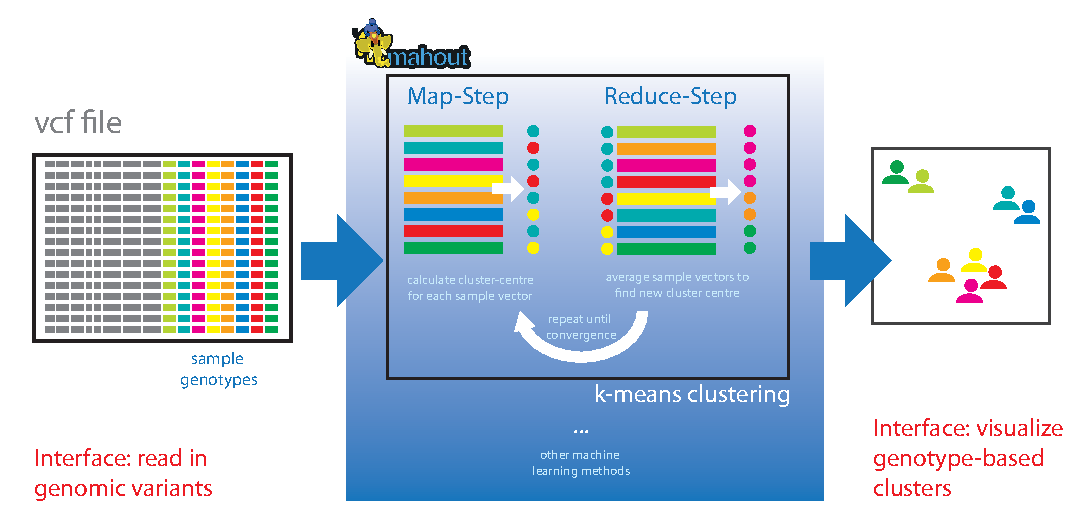
\includegraphics[type=pdf,ext=.pdf,read=.pdf, scale=0.40]{images/signature}
  \caption{\csentence{Illustration of Mahout-based clustering of genotypes.}
      The image shows how the here introduced interface converts the vcf file to a mahout usable vector-based data type. Based on k-means it illustrates how the Map-step procedure groups of vectors by their nearest cluster center and the Reduce-step averages the vectors in each group to find the new value of the updated cluster center. The mahout-produced output is then converted into a visualisation.}
      \end{figure}

\begin{figure}[h!]
  \caption{\csentence{Sample figure title.}
      Figure legend text.}
      \end{figure}

%%%%%%%%%%%%%%%%%%%%%%%%%%%%%%%%%%%
%%                               %%
%% Tables                        %%
%%                               %%
%%%%%%%%%%%%%%%%%%%%%%%%%%%%%%%%%%%

%% Use of \listoftables is discouraged.
%%
\section*{Tables}
\begin{table}[h!]
\caption{Datasets used in this study.}
      \begin{tabular}{lcc}
        \hline
           & individuals  & variants  \\ \hline
        \chrOnePop & 1092 & 816,115 \\
        \FullPop\ & 1092 & 38,219,238 \\
        \FullFam\ & 1092 & ...\\
      \end{tabular}
      \label{datasets}
\end{table}

\begin{table}[h!]
\caption{Adjusted Rand index (accuracy).}
      \begin{tabular}{lcccc}
        \hline
           & \chrOnePop & \FullPop  & hapmap \\ \hline
        Mahout, k=4 & 0.664 & ..&..\\
        Mahout, k=10 & 0.714 & ..&..\\
        Mahout, k=20 & 0.769 & .. & ..\\ 
        Mahout, k=30 & 0.728 & .. & ..\\ 
        R, k=4 & .. & - & -\\
        R, k=10 & .. & - & -\\
        R, k=20 & .. & - & -\\ 
        R, k=30 & .. & - & -\\ \hline
      \end{tabular}
      \label{datasetsAcc}
\end{table}

\begin{table}[h!]
\caption{Resources consumed.}
      \begin{tabular}{lccccc}
      \hline
      &&\multicolumn{2}{ c }{Memory (kb)}&\multicolumn{2}{ c }{Time (s)} \\
        \hline
           & Nodes & pmem & vmem  & pre-processing & clustering \\ \hline
        R, \chrOnePop & 1 & 17696940 & 18000196 &3341 & 7\\
        Mahout,\chrOnePop & 1 & 1831160 & 7646232 & 1255 & 594\\
        Mahout, \FullPop & .. &.. & .. & ..&..\\ 
        Mahout, 4 nodes & .. & .. & .. & ..&..\\ 
        \hline
      \end{tabular}
      \label{datasetsTime}
\end{table}


%%%%%%%%%%%%%%%%%%%%%%%%%%%%%%%%%%%
%%                               %%
%% Additional Files              %%
%%                               %%
%%%%%%%%%%%%%%%%%%%%%%%%%%%%%%%%%%%

\section*{Additional Files}
  \subsection*{Additional file 1 --- Sample additional file title}
    Additional file descriptions text (including details of how to
    view the file, if it is in a non-standard format or the file extension).  This might
    refer to a multi-page table or a figure.

  \subsection*{Additional file 2 --- Sample additional file title}
    Additional file descriptions text.


\end{backmatter}
\end{document}
